\section{Gestion des utilisateurs}\label{gestion-des-utilisateurs}

Unix est pensé pour supporter plusieurs utilisateurs. On doit d'abord
s'authentifier

\subsection{Authentification}\label{authentification}

On se connecte via un mot de passe en local ou distant (\emph{ssh}). Il
existe aussi les authentifications par données biométriques,
cryptographie asymétrique (private key and public key).

Le premier processus au démarrage est le processus de \texttt{login} qui
va lui fork tous les autres sous-processus. On liste tous les users dans
\texttt{/etc/passwd}. On y stockait avant les mots de passe dedans mais
maintenant on les stocke dans des fichiers séparés (\emph{shadow
password}).

\subsubsection{\texorpdfstring{\texttt{/etc/passwd}}{/etc/passwd}}\label{etcpasswd}

\texttt{oracle:x:1021:1020:Oracle\ user:/data/network/oracle:/bin/bash}

\texttt{1:2:3:4:5:6:7}

\begin{enumerate}
\def\labelenumi{\arabic{enumi}.}
\tightlist
\item
  Nom d'utilisateur
\item
  Mot de passe (stocké dans \texttt{/etc/shadow})
\item
  Identifiant User (\textbf{UID})
\item
  Identifiant du groupe \emph{principal} de l'user (\textbf{GID})
\item
  Informations supplémentaires, nom complet de l'user
\item
  Répertoire \emph{home}
\item
  Shell à exécuter au moment du login de l'user
\end{enumerate}

\subsubsection{Types d'user}\label{types-duser}

\begin{longtable}[]{@{}
  >{\centering\arraybackslash}p{(\columnwidth - 2\tabcolsep) * \real{0.1081}}
  >{\centering\arraybackslash}p{(\columnwidth - 2\tabcolsep) * \real{0.8919}}@{}}
\toprule\noalign{}
\begin{minipage}[b]{\linewidth}\centering
type d'user
\end{minipage} & \begin{minipage}[b]{\linewidth}\centering
Description
\end{minipage} \\
\midrule\noalign{}
\endhead
\bottomrule\noalign{}
\endlastfoot
root & Aucune restriction et peut tout faire. Admin du système. \\
User normal & Droit limité mais peut obtenir des droits de root via
\texttt{sudo}. \\
User système & Ne correspond pas un réel user mais correspond à des
services du SE. (typiquement des daemons, \ldots) \\
\end{longtable}

\paragraph{\texorpdfstring{Obtenir leur
\textbf{UID}}{Obtenir leur UID}}\label{obtenir-leur-uid}

On utilise la fonction \texttt{getuid(2)} pour obtenir l'\textbf{UID} et
\texttt{geteuid(2)} pour obtenir l'\emph{effective \textbf{UID}} car il
se peut que les droits changent temporairement (\texttt{sudo}).

\paragraph{\texorpdfstring{Changer
l'\textbf{UID}}{Changer l'UID}}\label{changer-luid}

On peut faire cela via \texttt{setuid(2)} qui modifie l'UID de
l'utilisateur en cours d'exécution. Donc Root appelle \texttt{setuid}
avant \texttt{execve} pour se donner les droits d'administration.

\section{Systèmes de fichiers}\label{systuxe8mes-de-fichiers}

Il y a énormément de diversité en terme de support de stockage de
données. Il faut donc une interface \emph{commune}. En \textbf{UNIX},
les fichiers sont regroupés sous forme d'une arborescence unique.

\subsection{Hiérarchie et Montage}\label{hiuxe9rarchie-et-montage}

\begin{figure}
\centering
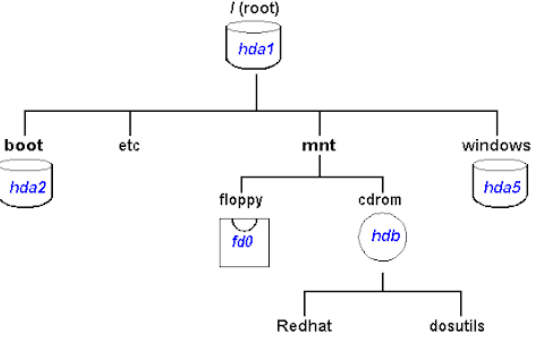
\includegraphics{image-34.png}
\caption{Alt text}
\end{figure}

En utilisant \texttt{mnt} on peut attacher ou détacher des systèmes de
fichiers dans la hiérarchie commune.

\subsection{contenu d'un répertoire}\label{contenu-dun-ruxe9pertoire}

\begin{verbatim}
$ ls -la / 
total 1488
drwxr-xr-x  19 root root    4096 Dec  9 14:35 .
drwxr-xr-x  19 root root    4096 Dec  9 14:35 ..
lrwxrwxrwx   1 root root       7 Apr 23  2020 bin -> usr/bin
drwxr-xr-x   2 root root    4096 Apr 23  2020 boot
drwxr-xr-x   9 root root    2820 Dec  9 14:35 dev
drwxr-xr-x 131 root root   12288 Dec  9 14:35 etc
drwxr-xr-x   3 root root    4096 Nov 15  2021 home
-rwxr-xr-x   3 root root 1440152 May  7  2022 init
lrwxrwxrwx   1 root root       7 Apr 23  2020 lib -> usr/lib
lrwxrwxrwx   1 root root       9 Apr 23  2020 lib32 -> usr/lib32
lrwxrwxrwx   1 root root       9 Apr 23  2020 lib64 -> usr/lib64
lrwxrwxrwx   1 root root      10 Apr 23  2020 libx32 -> usr/libx32
drwx------   2 root root   16384 Apr 10  2019 lost+found
drwxr-xr-x   2 root root    4096 Apr 23  2020 media
drwxr-xr-x   6 root root    4096 Sep 19 23:43 mnt
drwxr-xr-x   2 root root    4096 Apr 23  2020 opt
dr-xr-xr-x 244 root root       0 Dec  9 14:35 proc
drwx------   2 root root    4096 Feb 21  2023 root
drwxr-xr-x   6 root root     120 Dec  9 14:35 run
lrwxrwxrwx   1 root root       8 Apr 23  2020 sbin -> usr/sbin
drwxr-xr-x   2 root root    4096 Apr 10  2020 snap
drwxr-xr-x   2 root root    4096 Apr 23  2020 srv
dr-xr-xr-x  11 root root       0 Dec  9 14:35 sys
drwxrwxrwt  13 root root    4096 Dec  9 14:35 tmp
drwxr-xr-x  14 root root    4096 Apr 23  2020 usr
drwxr-xr-x  13 root root    4096 Apr 23  2020 var
\end{verbatim}

\subsubsection{Permissions}\label{permissions}

En analysant la première colonne, on peut savoir quelles sont les
permissions et si c'est un lien symbolique, hardlink ou directory.

On encode les permissions sur 9 bits via User (rwx), Groupe (rwx),
Autres (rwx). Ainsi, on connait les droits si on a le même UID, GUID ou
UID et GUID différents.

\begin{longtable}[]{@{}
  >{\centering\arraybackslash}p{(\columnwidth - 2\tabcolsep) * \real{0.0388}}
  >{\centering\arraybackslash}p{(\columnwidth - 2\tabcolsep) * \real{0.9612}}@{}}
\toprule\noalign{}
\begin{minipage}[b]{\linewidth}\centering
Droit
\end{minipage} & \begin{minipage}[b]{\linewidth}\centering
Description
\end{minipage} \\
\midrule\noalign{}
\endhead
\bottomrule\noalign{}
\endlastfoot
\texttt{r} & \emph{read}: lire le fichier, lister le contenu du
répertoire \\
\texttt{w} & \emph{write}: écrire dans le fichier, créer une entrée dans
le répertoire \\
\texttt{x} & \emph{execute}: accepter pour faire \texttt{execve} pour un
fichier. Pour un répertoire, on peut accéder à un fichier ou
sous-répertoire \\
\end{longtable}

\paragraph{\texorpdfstring{Subtilité du
\texttt{x}}{Subtilité du x}}\label{subtilituxe9-du-x}

\begin{verbatim}
$ mkdir -p repertoire 
$ echo "LINFO1252" > repertoire/fichier 
$ chmod 000 repertoire/ 
$ ls -al repertoire/
ls: cannot open directory repertoire/: Permission denied 
$ cat repertoire/fichier
cat: repertoire/fichier: Permission denied 
$ chmod +x repertoire/ 
$ ls -al repertoire/
ls: cannot open directory repertoire/: Permission denied
$ cat repertoire/fichier
LINFO1252
\end{verbatim}

\texttt{chmod} va changer les droits. On ne peut plus lister le fichier
car on a pas \texttt{r} mais on peut quand même y accéder car on a
\texttt{x} pour aller dans d'autres sous fichiers.

On représente les permissions comme 3 séquences de 3 bits donc
\texttt{rwxr-xr-\/-} = \texttt{754}. En utilisant \texttt{S\_ISUID} pour
un exécutable, permet l'exécution avec les permissions du propriétaire
de l'exécutable et pas celles de l'utilisateur.

\subsubsection{Navigation}\label{navigation}

Pour changer de répertoire en C où on exécute, on peut réaliser l'appel
suivant:

\begin{Shaded}
\begin{Highlighting}[]
\PreprocessorTok{\#include }\ImportTok{\textless{}unistd.h\textgreater{}}\PreprocessorTok{ }
\DataTypeTok{int}\NormalTok{ chdir}\OperatorTok{(}\DataTypeTok{const} \DataTypeTok{char} \OperatorTok{*}\NormalTok{path}\OperatorTok{);}
\end{Highlighting}
\end{Shaded}

\subsubsection{Fonctions Utiles}\label{fonctions-utiles}

\begin{longtable}[]{@{}
  >{\centering\arraybackslash}p{(\columnwidth - 2\tabcolsep) * \real{0.3070}}
  >{\centering\arraybackslash}p{(\columnwidth - 2\tabcolsep) * \real{0.6930}}@{}}
\toprule\noalign{}
\begin{minipage}[b]{\linewidth}\centering
Fonction
\end{minipage} & \begin{minipage}[b]{\linewidth}\centering
description
\end{minipage} \\
\midrule\noalign{}
\endhead
\bottomrule\noalign{}
\endlastfoot
\texttt{stat} & récupère les méta-données associées à un fichier ou
répertoire \\
\texttt{chmod}/\texttt{chown} & modifier les permissions ou le
propriétaire/groupe \\
\texttt{utime} & modifier les dates de création/modifications d'un
fichier (e.g.~commande \texttt{touch}) \\
\texttt{rename} & changer de nom, d'emplacement \\
\texttt{mkdir}/\texttt{rmdir} & créer/détruire un répertoire \\
\texttt{opendir}/\texttt{closedir}/\texttt{readir} & consulter le
contenu des répertoires \\
\end{longtable}

\subsubsection{Parcours de répertoire}\label{parcours-de-ruxe9pertoire}

\begin{Shaded}
\begin{Highlighting}[]
\KeywordTok{struct}\NormalTok{ dirent }\OperatorTok{\{} 
\NormalTok{    ino\_t d\_ino}\OperatorTok{;}                \CommentTok{/* inode number */}
\NormalTok{    off\_t d\_off}\OperatorTok{;}                \CommentTok{/* offset to the next dirent */} 
    \DataTypeTok{unsigned} \DataTypeTok{short}\NormalTok{ d\_reclen}\OperatorTok{;}    \CommentTok{/* length of this record */}
    \DataTypeTok{unsigned} \DataTypeTok{char}\NormalTok{ d\_type}\OperatorTok{;}       \CommentTok{/* type of file; not supported by all file system types */}
    \DataTypeTok{char}\NormalTok{ d\_name}\OperatorTok{[}\DecValTok{256}\OperatorTok{];}           \CommentTok{/* filename */}
\OperatorTok{\};}
\end{Highlighting}
\end{Shaded}

Il faut d'abord avoir ouvert un répertoire via \texttt{opendir}.
\texttt{readdir} pour accéder aux entrées du système.

TODO le reste
